\section{Object Detection Results}\label{sec:objectdetectionresults}

A total of 30 base trainings were performed. Sixteen training models used the medium-sized YOLOv8 pre-trained model, twelve used the large-sized YOLOv8 pre-trained model, and two trainings were conducted using the large-sized YOLO11 pre-trained model for comparison purposes. Since the YOLO11 pre-trained model series is an update of the YOLOv8 pre-trained model family, two experiments were conducted using only the best combination of hyperparameters found from the YOLOv8 base trainings. The detailed results, including the most important hyperparameters changed during the base training process and the main metric results, can be found in Tables A.1–6 in Appendix A.\\

Every base training varied in at least one hyperparameter. After each training process was completed, the resulting model was tested on the Mapillary Vistas testing subset, and the obtained metric values were saved. At the end, the 30 results were plotted against the training experiments (training ID). Figures 4.1, 4.2, and 4.3 show how some metrics (Precision, Recall, and mAP@50) varied across the 30 different training experiments. The best two models were selected after considering a balance between these results, with priority given to the mAP@50 and Recall metrics.

\newpage
\begin{figure}[h!]
    \centering
    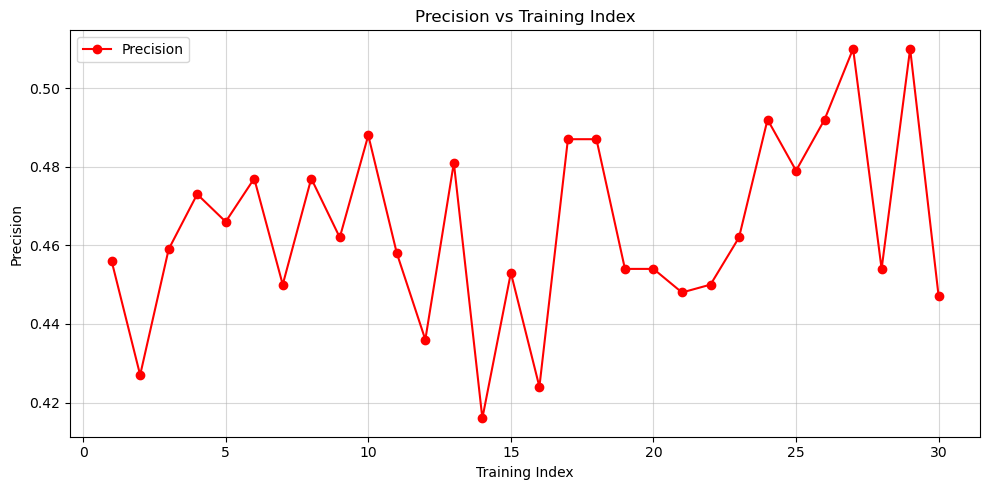
\includegraphics[width=0.8\textwidth]{src/images/bt_precision.png}
    \caption{Base Training Precision vs Training Index}
    \label{fig:bt1}
\end{figure}

\begin{figure}[h!]
    \centering
    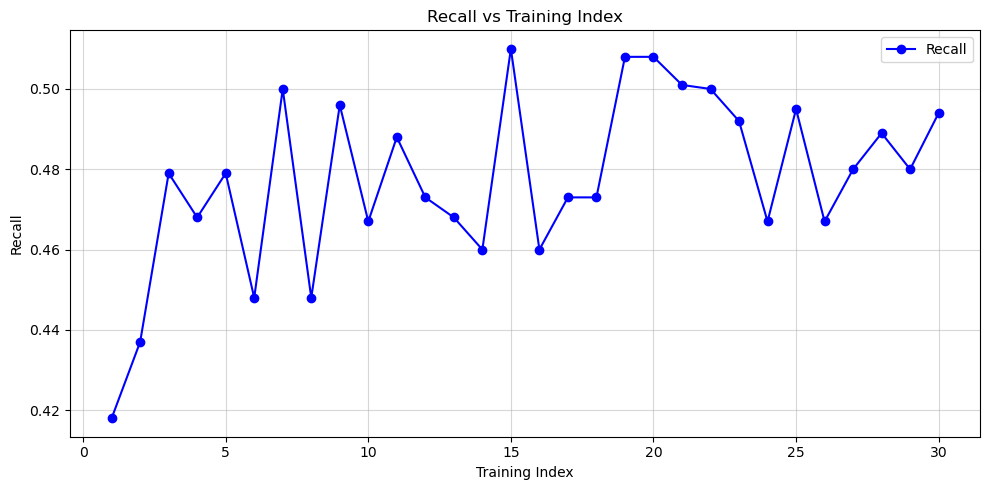
\includegraphics[width=0.8\textwidth]{src/images/bt_recall.png}
    \caption{Base Training Recall vs Training Index}
    \label{fig:bt2}
\end{figure}

\begin{figure}[h!]
    \centering
    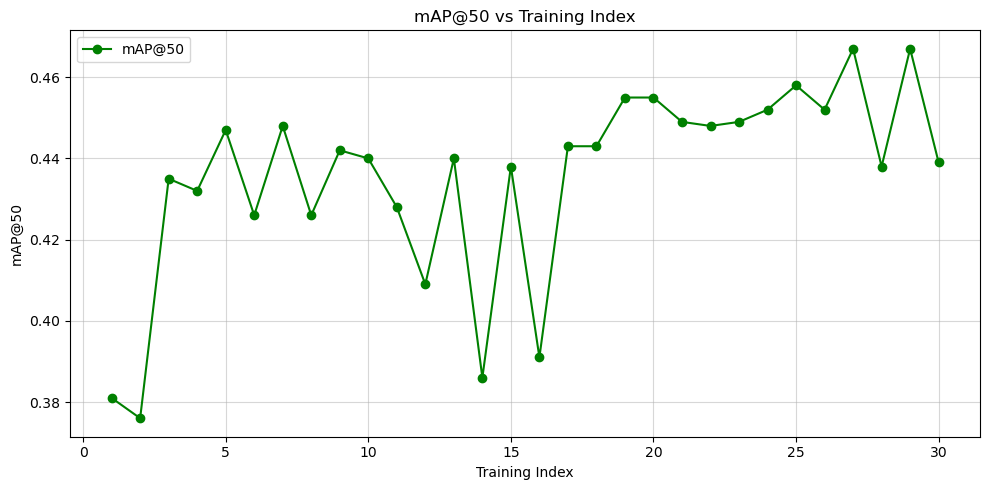
\includegraphics[width=0.8\textwidth]{src/images/bt_map50.png}
    \caption{Base Training map@50 vs Training Index}
    \label{fig:bt3}
\end{figure}

After careful consideration, experiments 19 and 27 (from the YOLOv8 and YOLO11 pre-trained models, respectively) were chosen based on their performance metrics. The details of their metric results can be found in Table 4.1.\\

\begin{table}[h!]
\centering
\renewcommand{\arraystretch}{1.3} % Adjust row height
\begin{tabular}{|c|c|c|}
\hline
\textbf{Metrics} & \textbf{Experiment 19 (v8)} & \textbf{Experiment 27 (11)} \\ \hline
\textbf{Precision} & 0.454  & 0.510  \\ \hline
\textbf{Recall} & 0.508   & 0.480  \\ \hline
\textbf{mAP@50} & 0.455   & 0.467  \\ \hline
\textbf{mAP@50-95} & 0.323  & 0.347  \\ \hline
\textbf{Fitness} & 0.337 &	0.347 \\ \hline
\end{tabular}
\caption{YOLOv8 and YOLO11 best base training experiments metric results.}
\label{tab:bestbasemetrics}
\end{table}

These two models were then fine-tuned using the BillboardLamac Dataset. A total of 20 fine-tuning experiments were conducted, with 10 per model. Once each fine-tuning experiment was complete, the resulting model was tested on the testing subset of the BillboardLamac Dataset. The same considerations as for the base training were taken into account, and the best two models were selected based on their metric performances. The complete fine-tuning results can be found in Tables A.7–10 in Appendix A. \\

Images 4.4, 4.5, and 4.6 show how metrics varied across the experiments, and Table 4.2 shows the details of the metrics for the 7th and 20th experiments (YOLOv8 and YOLO11 originally-based models), which were the best models identified after reviewing their results.\\

\begin{figure}[H]
    \centering
    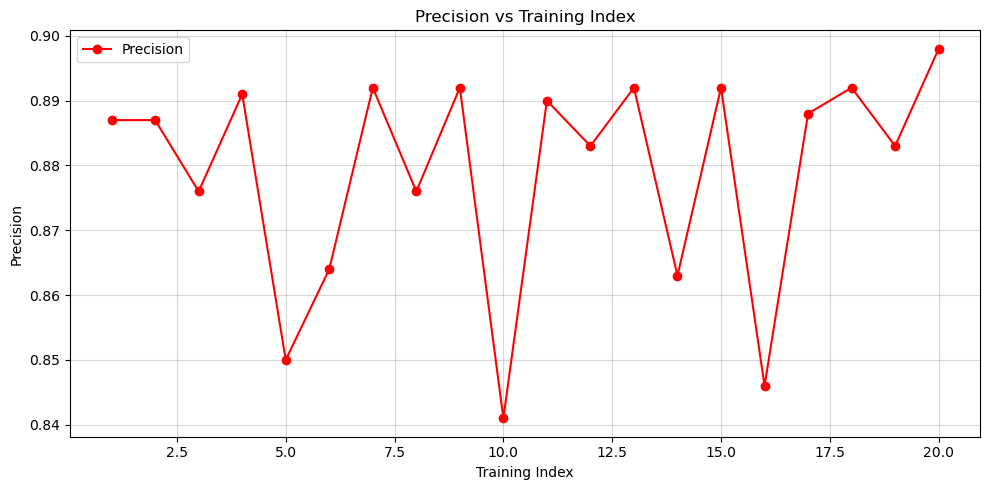
\includegraphics[width=0.8\textwidth]{src/images/ft_precision.png}
    \caption{Precision vs Training Index}
    \label{fig:ft1}
\end{figure}

\begin{figure}[H]
    \centering
    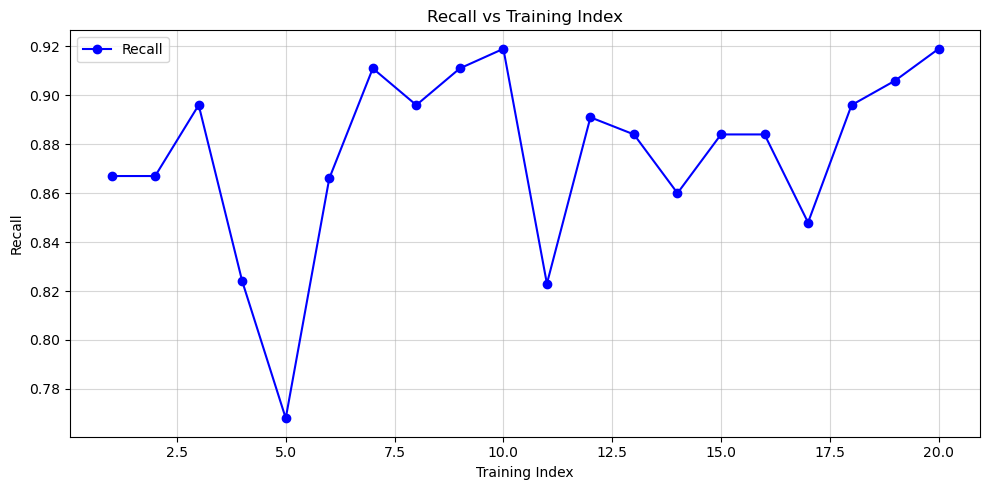
\includegraphics[width=0.8\textwidth]{src/images/ft_recall.png}
    \caption{Recall vs Training Index}
    \label{fig:ft2}
\end{figure}

\begin{figure}[H]
    \centering
    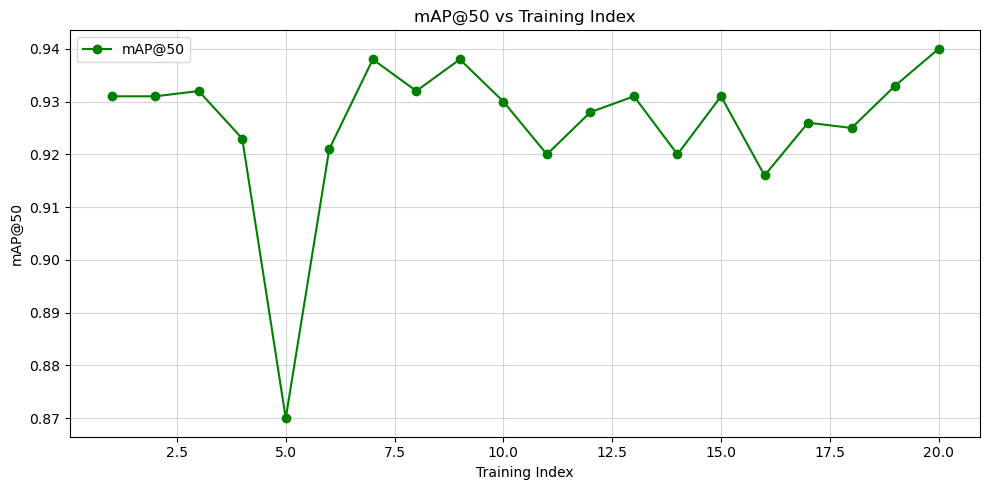
\includegraphics[width=0.8\textwidth]{src/images/ft_map50.png}
    \caption{map@50 vs Training Index}
    \label{fig:ft3}
\end{figure}

\begin{table}[h!]
\centering
\renewcommand{\arraystretch}{1.3} % Adjust row height
\begin{tabular}{|c|c|c|}
\hline
\textbf{Metrics} & \textbf{Experiment 7 (v8)} & \textbf{Experiment 20 (11)} \\ \hline
\textbf{Precision} & 0.892  & 0.898  \\ \hline
\textbf{Recall} & 0.911   & 0.919  \\ \hline
\textbf{mAP@50} & 0.938   & 0.940  \\ \hline
\textbf{mAP@50-95} & 0.771  & 0.794  \\ \hline
\textbf{Fitness} & 0.788 &	0.809 \\ \hline
\end{tabular}
\caption{YOLOv8 and YOLO11 best fine-tuning experiments metric results.}
\label{tab:bestfinetuningmetrics}
\end{table}